\section{Actors}\label{sec:processor-algorithm}
\subsection{Processor}\label{subsec:processor}
\begin{algorithm}[!ht]
    \DontPrintSemicolon
    \SetKwInput{KwInput}{Input}
    \KwInput{$G_{\phi}$: Scale weights from the Gate}
    \caption{~\emph{Processor Actor}: executed by a block}\label{alg:processor}
    \Begin{
        $tQ \gets \mathbf{GetTQ}()$\;
        $signal \gets 0$\;
        \tcp{shared memory variables}
        $task \gets \{\}$\;
        $interrupt \gets \kwFalse$\;
        $complete \gets \kwFalse$\;
        \While{$interrupt == $ \kwFalse}{
            \If{$warpId == 0$}{
                \If{$threadId == 0$}{
                    $\mathbf{awaitTaskFromScheduler}(interrupt,\>signal)$\;
                    $\mathbf{FencedNotifyRQ}(ready)$\;
                }
                $\mathbf{syncwarp}()$\;
                $\mathbf{warpReadTQ}(tQ, \>signal, \>task)$\;
            }
            $\mathbf{syncthreads}()$\;
            \If{$interrupt == $ \kwFalse}{
                \Switch{task.Type}{
                    \Case{$GEMM_0$}{
                        \tcp{fused GEMM, epilogue and async tile staging}
                        $\mathbf{fGET}(GEMM_0, \>task)$\;
                        \If{$threadId == 0$}{
                            $complete \gets \mathbf{NotifyTileCompletion}()$\;
                        }
                        $\mathbf{syncthreads}()$\;
                        \If{$complete == \kwTrue$}{
                            $\mathbf{NotifySchedulerNextGEMM}(tQ)$\;
                        }
                    }
                    \Case{$GEMM_1$}{
                        \tcp{fused GEMM, epilogue and async tile transfer}
                        $\mathbf{fGET}(GEMM_1, \>task)$\;
                    }
                    \Case{$Combine$}{
                        $\mathbf{combine}(task)$\;
                    }
                }
            }
        }
    }
\end{algorithm}
\clearpage
\subsection{Scheduler}\label{subsec:scheduler}
\begin{algorithm}[!ht]
    \DontPrintSemicolon
    \SetKwInput{KwInput}{Input}
    \SetKwBlock{DoParallel}{do in parallel}{end}
    \KwInput{$N$: Number of processors}
    \caption{~\emph{Scheduler Actor}: executed by one warp}\label{alg:scheduler}
    \Begin{
        $scheduled \gets 0$\;
        $tTB \gets 0$\;
        $tqState \gets \{\}$\;
        $pTDB \gets \mathbf{GetProcessorDoorbell}()$\;
        $sTDB \gets \mathbf{GetSubscriberDoorbell}()$\;
        $taskBound \gets \mathbf{GetTaskBound}()$\;
        $tTB \gets \mathbf{AtomicLoad}(taskBound)$\;
        \tcp{circular buffer ready queue}
        $rQ \gets \{\}$\;
        \tcp{Populate ready queue with Processor ids}
        $\mathbf{PopulateRQ}(rQ)$\;
        \While{$scheduled < tTB$}{
            $lt \gets 0$\;
            \DoParallel{
                $\text{Sweep doorbells and populate observed task counts into } tqState$\;
                $\text{Aggregate locally observed task counts into } lt$\;
            }
            $qS,\>taskTally \gets 0$\;
            \tcp{qS is the inclusive output}
            $\mathbf{WarpInclusiveSum}(lt, qS, tasktally)$\;
            \While{$tasktally > 0$}{
                $\text{Repopulate } rQ \text{ with ready processor ids}$\;
                \DoParallel{
                    $\text{Starting at } rQ[qS] \text{, signal processors about task indices from } tqState$
                }
            }
            \If{$threadId == 0$}{
                $tTB \gets \mathbf{AtomicLoad}(taskBound)$\;
            }
            $tTB \gets \mathbf{WarpBroadcast}(tTB)$
        }
        $\mathbf{InterruptSubscribers}()$\;
        $\mathbf{InterruptProcessors}()$\;
    }
\end{algorithm}
\clearpage
\subsection{Subscriber}\label{subsec:subscriber}
\begin{algorithm}[!ht]
    \DontPrintSemicolon
    \SetKwBlock{DoParallel}{do in parallel}{end}
    \SetKwInput{KwInput}{Input}
    \KwInput{$O \in \mathbb{R}^{S \times H}$, $X \in \mathbb{R}^{E\times H \times P}$}
    \caption{~\emph{Subscriber Actor}: executed by three warps}\label{alg:susbcriber}
    \Begin{
        $interrupt \gets \mathbf{GetSharedInterrupt}()$\;
        $flags \gets \mathbf{GetSymmetricFlags}()$\;
        $tQ \gets \mathbf{GetTQ}()$\;
        \tcp{Predefined upper bound on the number of tasks.}
        \tcp{We modulate this value to the actual task count computed}
        \tcp{dispatch signals received from peer GPUs}
        $taskBound \gets \mathbf{GetTaskBound}()$\;
        \While{$\mathbf{AtomicLoad}(interrupt) == $ \kwFalse}{
            \tcp{dispatch flags}
            \DoParallel{
                $\text{Visit dispatch flags}$\;
                $\text{Atomically retrieve signal}$\;
                \If{$\text{Signal is set and flag is not visited}$}{
                    $\text{Mark visited}$\;
                    $\mathbf{SelfCorrectTaskBound}(taskBound, Signal)$\;
                    $\text{Enforce memory consistency before consuming packet}$\;
                    $\text{Decode packet into a set of } GEMM_0 \text{ task descriptors using } X$\;
                    $\text{Write task descriptors to } tQ$\;
                    $\text{Notify Scheduler of decoded tasks}$\;
                }
            }
            $\text{Advance flags by number of dispatch flags length}$\;
            $\text{Atomically retrieve signal}$\;
            \tcp{combine signals}
            \DoParallel{
                $\text{Visit combine flags: one per tile}$\;
                \If{$\text{Signal is set and flag is not visited}$}{
                    $\text{Mark visited}$\;
                    $\text{Enforce memory consistency before consuming packet}$\;
                    $\text{Decode packet into a set of } combine \text{ task descriptors using } O$\;
                    $\text{Write task descriptors to } tQ$\;
                    $\text{Notify Scheduler of decoded tasks}$\;
                }
            }
        }
    }
\end{algorithm}
\clearpage
\section{Multi-Node Evaluation}\label{sec:multi-node-evaluation}
\subsection{Setup}\label{subsec:setup}
In this experiment, we seek to evaluate \sysname in the multi-node setting.
We use 4 nodes, where each node comprises 4 A100 GPUs fully interconnected via NVLink.
Across nodes, each GPU uses a single NIC providing 25 GB/s of bandwidth.
We set the number of experts to be $16$ and assign each GPU to host only one,
so the number of local experts is $1$.
Note that we define MIV formally as follows:
\[
    MIV = \frac{Tokens}{Experts} * local\_{experts} * precision * hidden\_size * 2 * n_{rg}
\]
where $n_{rg}$ is the number of remote peers and the multiplicative
factor of $2$ accounts for communication rounds (dispatch and combine).
$n_{rg} = 12$ for this experiment.
\subsection{Results}\label{subsec:results}
\begin{figure} [!ht]
    \centering
    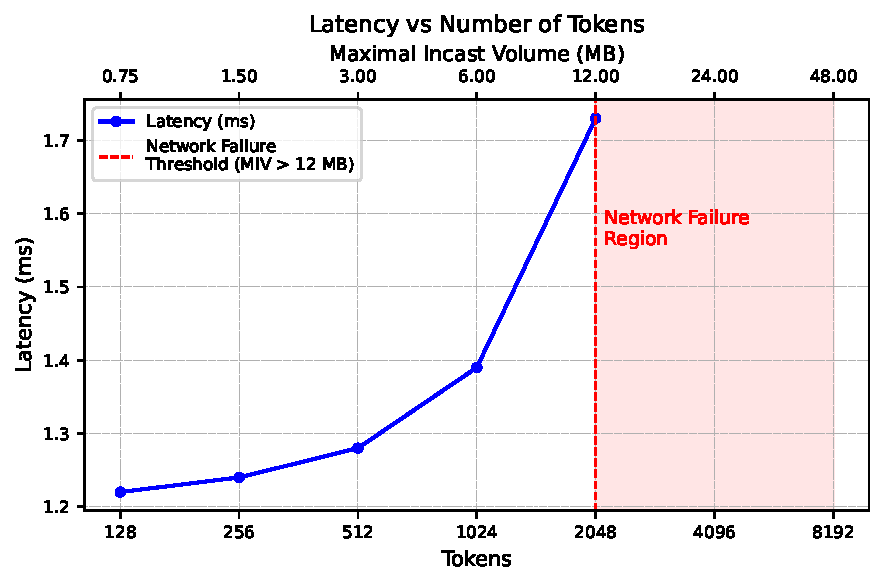
\includegraphics[width=4in,keepaspectratio]{figures/multi_node_fail}
    \caption{Multi-node Latency evaluation.
    Embbeding dimension is $1024$ and FFN intermediate size is $4096$.
    We define Maximal Incast Volume (MIV) as the worst case upper bound for data volume that a
    NIC receives in a single incast occurence.}
    \label{fig:multi_fail}
\end{figure}
We observe a sublinear increase in latency as we scale the number of tokens.
However, we observe at $Tokens > 2048$, that the application fails to terminate
due to failure to receive expectant messages.
We hypothesize this failure to be due to buffer overflow at the networking hardware layer as is common for applications
that generate many and large messages~\cite{nerscNetworkNERSC} like our system.
We note that this failure is addressable by tuning hardware configurations~\cite{ofiwgFi_cxi7} but we consider
this exploration as an exercise orthogonal to this work.
\clearpage